%
%

%%-----------------------------------------------------
%%-----------------------------------------------------
\section{¿Qué datos tuyos tienen?}

%%-----------------------------------------------------
\begin{frame}
\frametitle{Un ejemplo: Facebook}

\begin{columns}[T]
\begin{column}{.65\textwidth}
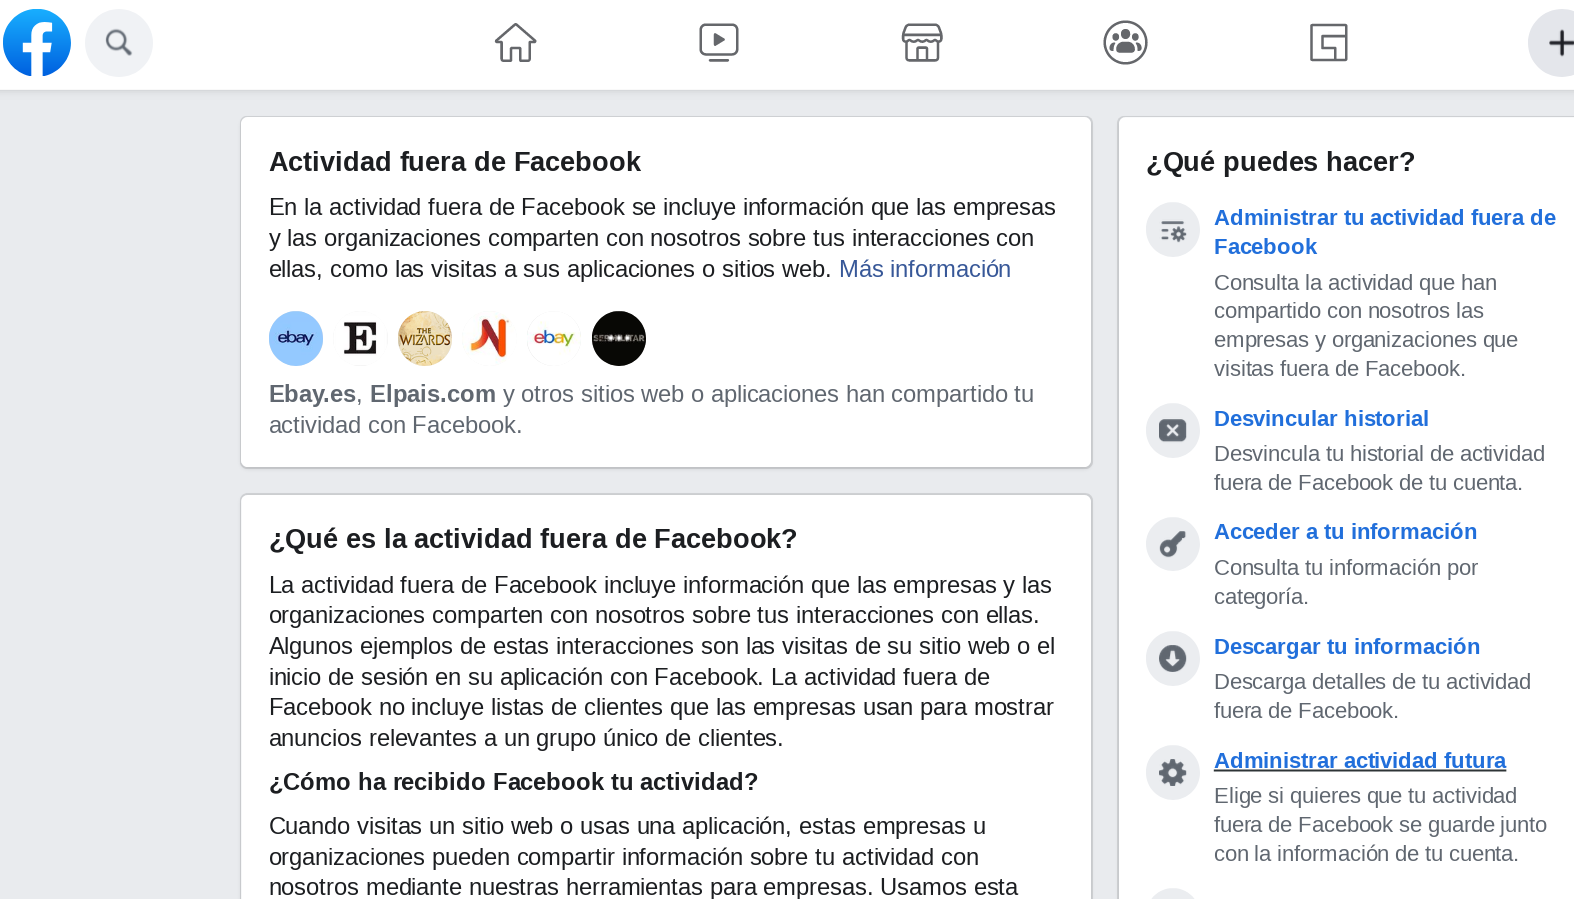
\includegraphics[width=8cm]{figs/facebook-offsite}

\begin{flushright}
{\footnotesize
\url{https://www.facebook.com/off_facebook_activity}
}
\end{flushright}

\end{column}%
\hfill%
\begin{column}{.32\textwidth}
  Puedes consultar la información que Facebook tiene sobre ti...

  ...conseguida cuando estabas fuera de Facebook

  (gracias a los trackers de Facebook)
\end{column}%
\end{columns}

\end{frame}


%%-----------------------------------------------------
\begin{frame}
  \begin{center}
    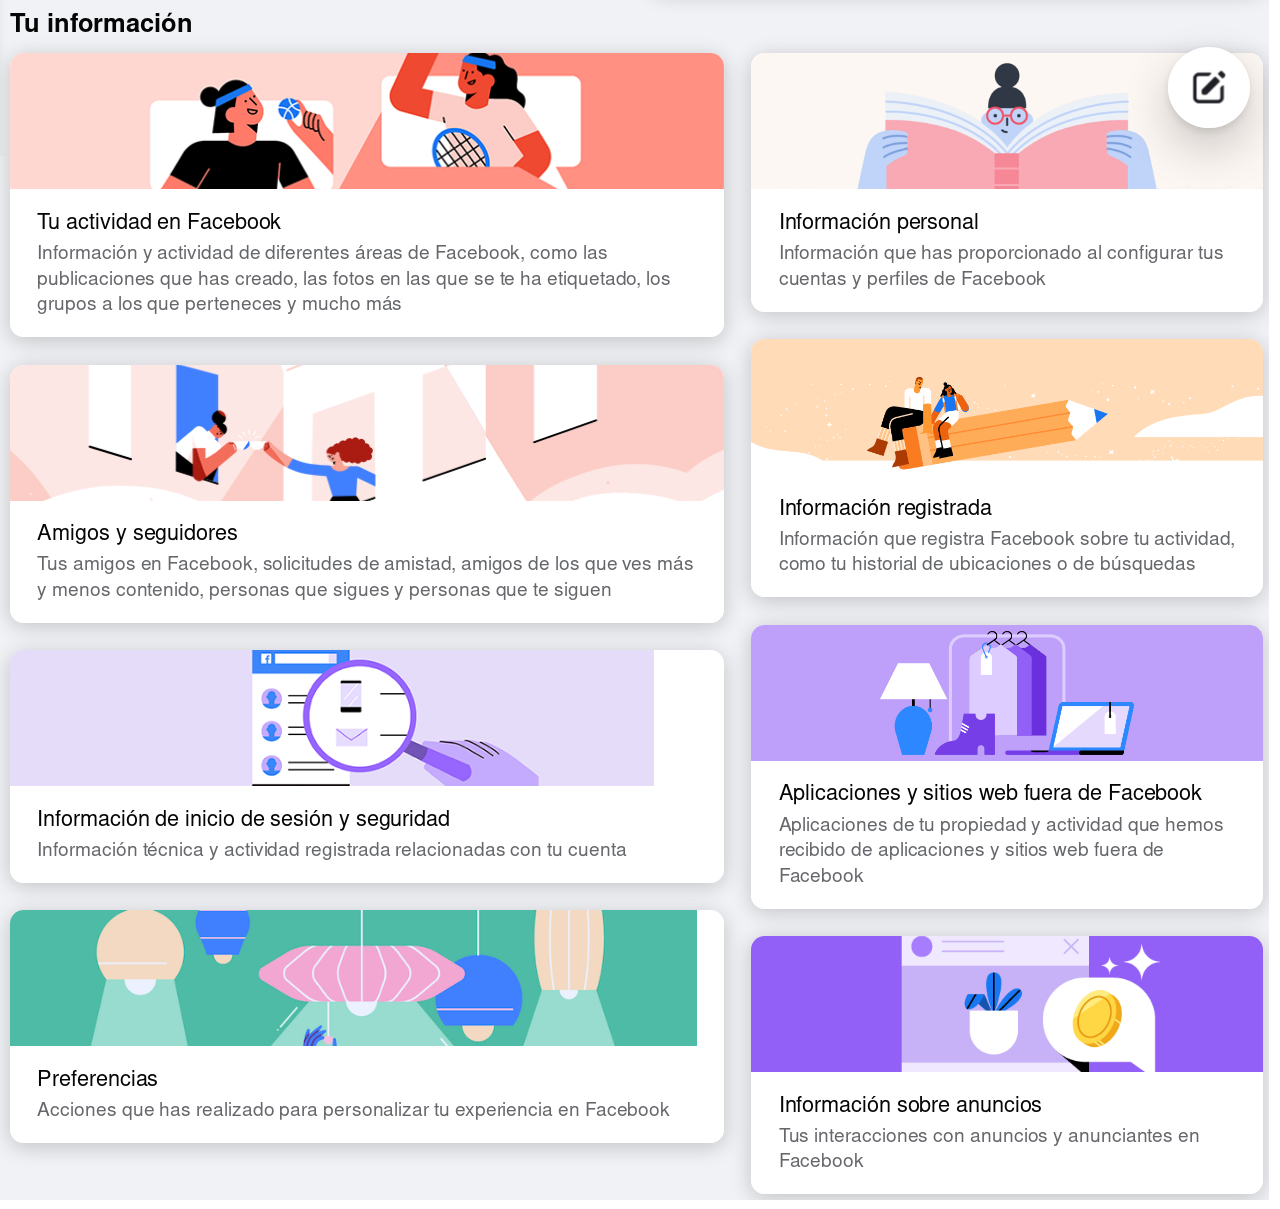
\includegraphics[width=8cm]{figs/facebook-offsite-2}
  \end{center}
\end{frame}


%%-----------------------------------------------------
\begin{frame}
  \frametitle{Más casos}

  {\Large
    
    Google:

    \begin{flushright}
      \url{https://myactivity.google.com}
    \end{flushright}

    Microsoft:
    
    \begin{flushright}
    \url{https://account.microsoft.com/privacy}
    \end{flushright}

    Amazon:
    
    \begin{flushright}
      \url{https://www.amazon.com/gp/help/customer/display.html?nodeId=GXPU3YPMBZQRWZK2}
    \end{flushright}
  }
\end{frame}

%%-----------------------------------------------------
\begin{frame}
  \frametitle{GDPR}

  \begin{center}
    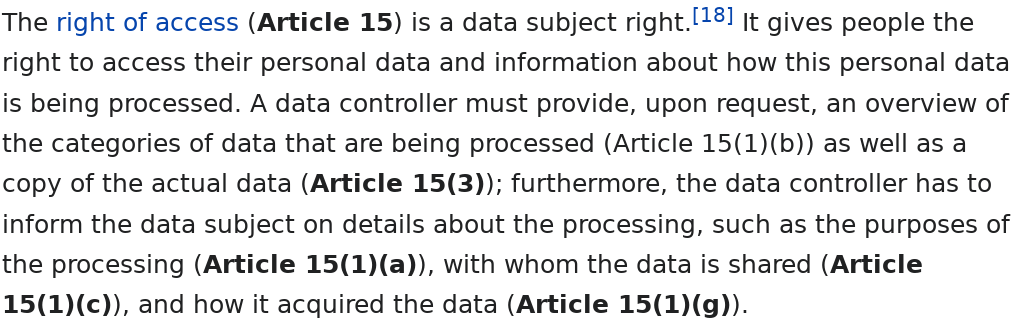
\includegraphics[width=12cm]{figs/gdpr}
  \end{center}

  \vspace{.5cm}
  
  {\Large  
    General Data Protection Regulation:
  }

  \begin{flushright}
    {\small
      \url{https://en.wikipedia.org/wiki/General_Data_Protection_Regulation}
      }
    \end{flushright}

\end{frame}
